\section{Weather Monitoring System}
% wms.viwetter.de
% Was ist WMS BEGIN
Das \textit{Weather Monitoring System} (kurz WMS) beschreibt eine Reihe von Bildschirmen die verteilt in Kühlungsborn Grafiken eines zentralen Servers anzeigen sollen.
Diese Grafiken enthalten generelle Informationen über Kühlungsborn,
sowie Wetterdaten und Wetterprognosen.
Im Schulzentrum Kühlungsborn findet man eine weitere Anwendung des WMS. \\
Im Foyer sollen Bildschirme Grafiken von Schülern für Schüler zeigen.
Diese Grafiken beinhalten Geburtstagswünsche, Termine, oder allgemeine Fakten zu aktuellen Geschehnissen. \\
Die Domain über die die Rechner den WMS-Server erreichen ist \link{http://wms.viwetter.de}.
Auch wenn dieser von überall aus erreichbar ist,
muss man sich authentifizieren um Daten zu bearbeiten oder anzuzeigen.\\
Im letzten Jahr der Projektarbeit stellte sich das Weather Monitoring System als
interessante Baustelle heraus. Dieses wurde von Grund auf neu entwickelt und integriert.
% Was ist WMS ENDE

\subsection{Konzept} % WMS
Schüler sollen in der Lage sein die von ihnen in der Projektarbeit erzeugten Grafiken über ein möglichst einfaches Interface auf einen Server zu laden.
Sie sollen anschließend die Bilder ersetzen bzw. löschen können.
Damit die Serveradministrator, in diesem Fall \mb und \re ,
bestimmen können wer für welchen Ordner Grafiken hochladen und einbetten kann ist der Zugriff auf die Dateimanagementfunktion nur über ein Benutzerkonto möglich.
Es können von jedem Administrator nach Bedarf neue Konten erstellt werden. \\
Auch zum anschauen der Grafiken muss man ein Konto besitzen,
allerdings soll der Anzeigecomputer auch von alleine in der Lage sein sich einzuloggen und die Grafiken eines voreingestellten Ordners anzeigen.
Zum Anzeigen muss eine Authentifizierung stattfinden,
da Schüler zum einen manchmal unwissend Grafiken mit Copyright hochladen,
und sich die Serveradmins und Webadmins schützen und auch den
Schülern etwas entgegenkommen wollen. \\
Auch bei diesem Interface greift natürlich die Regel,
dass auch ein Affe die Datenbank bedienen können soll
und auch die obligatorische Katze auf der Tastatur soll das
System nicht zum Absturz bringen. \footnote{diese Regel gibt dem System
dessen Namen ,,apewms'' auf Github.com}

\subsection{Hardware}
Zum Weather Monitoring System gehören zwei Bereiche die mit Hardware etwas zutun haben.
Einerseits muss es einen Server geben, welcher die Daten bereitstellt,
und gleichzeit auch möglichst interaktiv das Bearbeiten und Hochladen von neuen Daten ermöglicht.
Diesem Server sollte genügen Speicherplatz bereitstehen,
um alle Grafiken zu speichern.
Aus der Spezifikation, dem Konzept, kann man schon ablesen, dass auch eine Datenbank auf dem
Server angelegt werden muss.\\
Der Client des Weather Monitoring Systems, muss funktionell nur Grafiken auf einem Bildschirm anzeigen.
Diese Aufgabe ist nicht alzu aufwendig,
daher ist bei der Auswahl der Clienthardware robustheit ein wichtigerer Faktor.
Außerdem sollte die Hardware, noch eher als beim Server, möglichst kostgünstig sein,
da früh eingeplant werden mussten,
bei einem funktionierenden System mehrere Anzeigen einzusetzen.
Die Lösung für Server und Client fand sich mit dem Raspberry Pi.
Dieser kleine Rechner wurde für diese Arbeit schon mehrmals als Lösung herangezogen,
und durch die Verfügbarkeit,
Erfahrung mit der Hardware sowie der Möglichkeit direkt Prototypen
zu testen bot es sich an einen Raspberry Pi als Server und Client zu benutzen.\\
Für beide Anwendungsfälle wurde eine abgewandelte
Version des Raspbian Betriebssystems zusammengestellt
um die verlangte Aufgabe bestmöglichst zu erfüllen.


\subsection{Interface} % WMS
Nachdem ein Nutzer die Anmelderoutine durchgeführt hat wird ihm die Struktur der Daten nach Anzeigeindex geordnet angezeigt.
Der Nutzer, in diesem Fall der Schüler oder der Endnutzer am Bildschirm,
selbst hat nur einen geringen Einblick in die Datenbank, und kann nicht direkt auf den Ordner auf dem Server zugreifen.\\
Das bereitgestellte Interface ermöglicht dem Nutzer aber neue Ordner
zu erstellen und Grafiken hochzuladen und zu löschen.
Dabei wird im Hintergrund von jedem Bild der Autor gespeichert. \\
Das Interface selbst ist hauptsächlich in PHP und CSS geschrieben.
Natürlich ist ein gewisser Grad von JavaScript und HTML unumgänglich. \\
Da auch die Bearbeitung der Daten von einem Raspberry Pi möglich sein soll ist der HTML Code nicht an der vordersten Front der HTML Syntax (zum Zeitpunkt der Setzung HTML5),
sondern beruht auf grundlegenden Elementen und enthält auch kaum Animationen. \\
JavaScript wird nur benutzt um Eingabeformulare auf offensichtliche Fehler zu überprüfen.
Außerdem schränkt das Interface den Nutzer bewusst ein,
sodass die Wahrscheinlichkeit,
dass er etwas veranlasst, wovon er nicht wusste was es bewirkt, verringert wird.
Außerdem kann er selbst mutwillig nicht das gesamte System zum Absturz bringen.
Dies beinhaltet das Freigeben des Links um die Anzeige einzuschalten,
dies kann nur durch einen Admin geschehen.
Auch der Schüler soll vor sich selbst geschützt werden.
Es ist ihm nicht möglich einen Link als Grafik hochzuladen,
oder eine Offlinedatei zu Verlinken.
Wenn der Nutzer auswählt eine Grafik hochzuladen,
hat er nicht die Möglichkeit eine Verlinkung einzufügen, und vice versa.
\begin{center}
    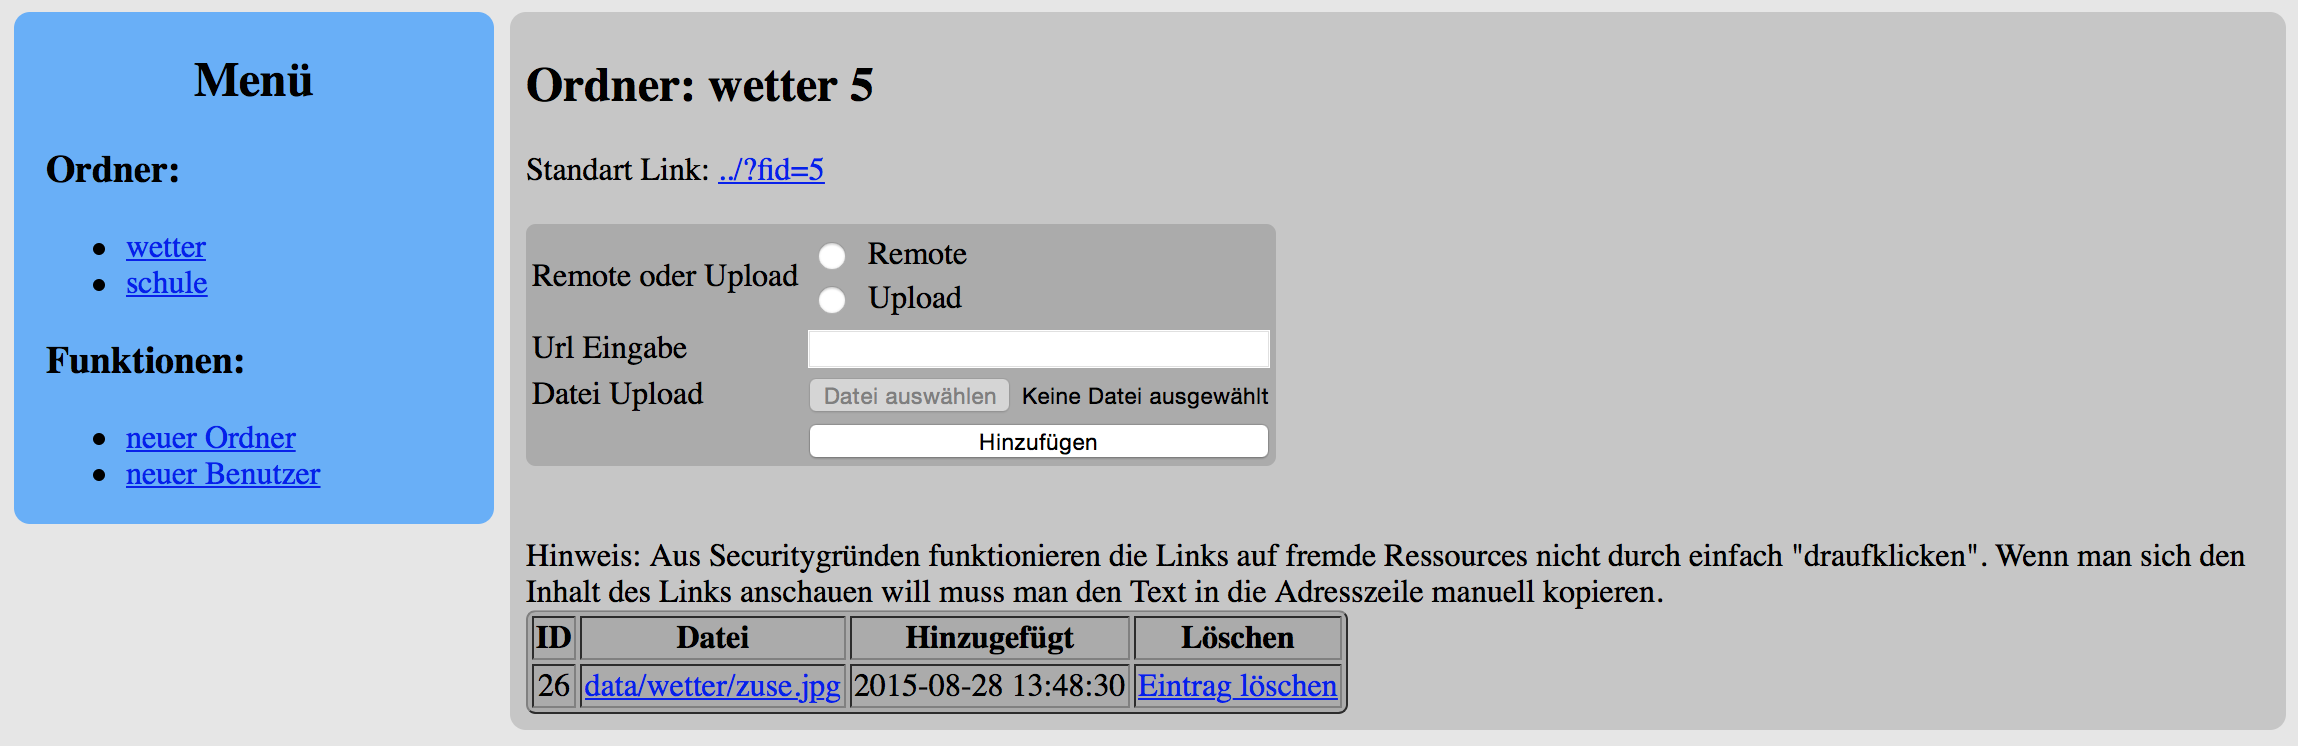
\includegraphics[width=\linewidth]{imgs/wms/wms_interface.png}
\end{center}
Diese Grafik zeigt das Erscheinungsbild des WMS-Interfaces. Es ist sichtbar
minimalistisch gehalten um robust zu sein, und auch die Wartung zu erleichtern.
Trotzdem ist es dynamisch, denn es erlaubt die Erstellung neuer Ordner und Nutzer,
und in allen Testszenarien konnte die Seite nicht zum Absturz gebracht werden.

\subsection{Generierte Grafiken}
\label{sub:Generierte Grafiken}
In diesem Abschnitt der Projektarbeit bestand wieder ein Bedarf nach automatisiert erzeugten Grafiken.
Einerseits ist das Wetter, ,,Weather'' ja schon namensgebend, somit ist der \vs -Teil meiner Arbeit schon relevant.
Zudem fand sich aber auch ein anderer Anlass Grafiken automatisiert zu generieren.
Das WMS System befindet sich im Foyer des Schulzentrum Kühlungsborns in dreifacher Ausführung.
Einer der Rechner soll als Geburtstagsanzeige genutzt werden.
Er zeigt also eine Reihe von Grafiken an, auf denen grafisch aufbereitete Tabellen aus Namen und Geburtsdaten der aktuellen Woche zu sehen sind.
Die Erzeugung dieser Grafiken erfolgte historisch im Hafen im Rahmen des Wahlpflichtfaches unter der Leitung von Dr. Ronald Eixmann.
Die Arbeit ist zeitaufwändig, und ein Schüler muss angelernt werden wie CoralDraw bedient wird.
Auch wenn die Fähigkeit dieses Programm benutzen zu können nicht unwichtig ist, ist die Arbeit die
Daten aus einer Tabelle zu lesen und in eine Maske einzutragen nicht notwendigerweise von einem Menschen abhängig.\\

\subsection{Application Programming Interface}
\label{sub:wmsapi}
Ein Application Programming Interface, kurz API, ist eine Schnittstelle zu einem größeren Programm
über eine Programmiersprache, welche nicht der des ursprünglichen Programmes entsprechen muss.
Über diese Schnittstelle soll dann die Ausführung von Aufgaben veranlasst werden.
Eine API ermöglicht also dann Entwicklern auf ihr Programm von außen zuzugreifen und es zu erweitern.
In dem Fall von WMS war eine API notwendig um von Programmen aus,
also nicht von \link{wms.viwetter.de}, Grafiken hochzuladen und zu verwalten.
Im Detail wird die API genutzt um die erzeugtet Geburtstagsgrafiken von einem Python Programm auf den Server zu laden und die Geburtstagsgrafikenschleife zu verwalten.
Die API auf Seiten des Servers ist in PHP geschrieben.
Auf diese API kann nun von außen jede Programmiersprache über GET und POST Requests des Hyper Text Transfer Protokolls zugreifen.
Eine dieser Programmiersprachenschnittstellen wurde für Python geschrieben.\\
Dieses System emuliert Großteils das REST-Ful Paradigmus.

\subsection{Erreichbarkeit} % WMS
Auch wenn der Server nicht globales Interesse erweckt soll er natürlich nicht nur im Hafen erreichbar sein.
Da Standorte sich auch verändern können,
und nicht dringend immer in Kühlungsborn liegen müssen, ist der Server über den Domainnamen \link{http://wms.viwetter.de} erreichbar. \\
Alle Funktionen die hier beschrieben wurden sind demnach auch von jedem internetfähigen PC erreichbar. Keiner der Computer hat Sonderrechte,
und es werden auch keine Cookies gespeichert.

\subsection{Sicherheit} % WMS
Da dieses System an öffentlichen Orten Anwendung finden soll,
muss gewährleistet sein, dass auf den Anzeigegeräten nur Daten angezeigt werden,
die von autorisierten Personen ausgewählt worden.
Außerdem soll der Service nicht ohne die Erlaubnis eines Administrators aufrufbar sein,
deshalb wurde ein Kontensystem implementiert.
Da die Client Computer automatisiert starten und gleich die richtigen Daten anzeigen sollen,
musste ein Protokoll entwickelt werden, welches sicher ist,
aber einem entferntem Rechner ermöglicht sich selbst anzumelden.
Um dafür zu sorgen, dass nur vollständig geladene Grafiken angezeigt werden muss
der Client beim Anzeigen selbst überprüfen ob die Grafik vorhanden ist.
Um sicherzustellen, dass die Anzeige auch im Rahmen der Projektarbeit aufgestellt
wurde muss sich der Rechner selbst authentifizieren.
Dafür muss auf ihm lokal ein Benutzername und ein
Authentifizierungshash gespeichert sein. Sein Passwort im Klartext ist dem Server nicht bekannt.
Selbst wenn der gesamte Datenbankinhalt veröffentlicht wird, kann weder ein Passwort
entschlüsselt werden\footnote{zumindest in einer Zeitspanne die
geringer als die Lebensdauer des Universums ist}, noch können Nutzer die das selbe Passwort haben
gruppiert werden.\\
Dieses Verhalten wurde erreicht indem das Passwort zusammen mit einem ,,Salt''-Wert gehash wird.
Dieser ,,Salt'' wird bei jedem Benutzer individuell
erzeugt und ist eine 256 Bit lange zufällige hexdezimale Zeichenkette.\\
Nicht nur der Server muss vor Angriffen geschützt werden, sondern auch der
Nutzer am anderen Ende der Leitung.
Teile des Interfaces nutzen JavaScript.
Diese Programmiersprache kann genutzt werden um Angriffe durchzuführen, und
auf jeder Seite die dynamische Inhalte anbietet gibt es die Gefahr das ein
Cross-Site-Scripting Angriff möglich ist.
Auf dem WMS-Interface wurden alle Vorbereitungen getroffen, dass dies nicht der
Fall ist. Jede Anfrage die dem Server geschickt wird, wird bevor sie in die Datenbank
geschrieben wird escaped. Escaping ist der Vorgang in dem Zeichen, die für den
Computer in einer Programmiersprache eine besondere Bedeutung haben so zu kennzeichnen,
dass sie nur als ,,Text'' gelesen und verstanden werden.
Um dann SQL-Injektionen zu verhindern werden alle Interaktionen mit der Datenbank
nicht über ,,normale'' SQL-Queries gehandhabt, sondern über Prepared-Statements
dürchgeführt.
\lstinputlisting[language=PHP]{example/prepared.php}
Ein Prepared Statement ist in SQL eine Befehlstruktur, in der Befehl und Inhalt
über zwei komplett getrennte Verbindungen transferiert werden.
Eine SQl-Injektion in der Form:
\lstinputlisting[language=PHP]{example/sqlinject.php}
kann nicht nur für Datenverlust, sondern auch für die Veröffentlichung
von Passwörtern und privaten Daten sorgen. Durch die Trennung von Befehl und Inhalt,
kann also mit geringfügig mehr Aufwand die Datensicherheit erheblich verbessert werden.
Aus diesem Grund werden serverseitig nur\footnote{Über Prepared Statements
können einige Daten nicht übertragen werden, an wenigen Stellen wird auf altmodische
Queries zurückgegriffen} Prepared Statements eingesetzt.

\subsection{Anzeige}
Die Anzeige erfolgt über den Browser, da ein Internetbrowser meist vorinstalliert ist
und die meisten Medien nativ anzeigen kann, ohne das ein zusätzliches Software packet
benötigt. \\
Nur einen Browser zu starten reicht allerdings nicht um das von mir verlangte Verhalten
zu erreichen. Der Browserstart soll direkt nach dem Bootvorgang erfolgen, der Rechner soll
dann auch so robust eingerichtet sein, dass sein Dateisystem bei dem wildesten Stromnetz
noch funktionsfähig bleibt.\\
Für diesen Zweck wurde eine abgewandelte Version des Open Source Raspbian Betriebssystems
entwickelt, das diesen Schritt automatisiert ausführt. Bei der Installation des
Rechners muss nur das Ziel eingegeben werden und die restliche Konfiguration
übernimmt das System. Um einem Rechner dieses Betriebssystem zu überspielen wird
wieder ein Raspberry Pi genutzt für den das Betriebssystem auf eine SD-Karte über
den Linux dd Befehl überspielt wird. Von dieser SD-Karte kann der Raspberry Pi
ohne Konfiguratin booten und die Einstellung des Ziels der Anzeige kann über eine
Tastatur an dem Pi selbst oder über eine SSH Verbindung erledigt werden.
